% Options for packages loaded elsewhere
\PassOptionsToPackage{unicode}{hyperref}
\PassOptionsToPackage{hyphens}{url}
\PassOptionsToPackage{dvipsnames,svgnames,x11names}{xcolor}
%
\documentclass[
  letterpaper,
  DIV=11,
  numbers=noendperiod]{scrartcl}

\usepackage{amsmath,amssymb}
\usepackage{lmodern}
\usepackage{iftex}
\ifPDFTeX
  \usepackage[T1]{fontenc}
  \usepackage[utf8]{inputenc}
  \usepackage{textcomp} % provide euro and other symbols
\else % if luatex or xetex
  \usepackage{unicode-math}
  \defaultfontfeatures{Scale=MatchLowercase}
  \defaultfontfeatures[\rmfamily]{Ligatures=TeX,Scale=1}
\fi
% Use upquote if available, for straight quotes in verbatim environments
\IfFileExists{upquote.sty}{\usepackage{upquote}}{}
\IfFileExists{microtype.sty}{% use microtype if available
  \usepackage[]{microtype}
  \UseMicrotypeSet[protrusion]{basicmath} % disable protrusion for tt fonts
}{}
\makeatletter
\@ifundefined{KOMAClassName}{% if non-KOMA class
  \IfFileExists{parskip.sty}{%
    \usepackage{parskip}
  }{% else
    \setlength{\parindent}{0pt}
    \setlength{\parskip}{6pt plus 2pt minus 1pt}}
}{% if KOMA class
  \KOMAoptions{parskip=half}}
\makeatother
\usepackage{xcolor}
\setlength{\emergencystretch}{3em} % prevent overfull lines
\setcounter{secnumdepth}{-\maxdimen} % remove section numbering
% Make \paragraph and \subparagraph free-standing
\ifx\paragraph\undefined\else
  \let\oldparagraph\paragraph
  \renewcommand{\paragraph}[1]{\oldparagraph{#1}\mbox{}}
\fi
\ifx\subparagraph\undefined\else
  \let\oldsubparagraph\subparagraph
  \renewcommand{\subparagraph}[1]{\oldsubparagraph{#1}\mbox{}}
\fi

\usepackage{color}
\usepackage{fancyvrb}
\newcommand{\VerbBar}{|}
\newcommand{\VERB}{\Verb[commandchars=\\\{\}]}
\DefineVerbatimEnvironment{Highlighting}{Verbatim}{commandchars=\\\{\}}
% Add ',fontsize=\small' for more characters per line
\usepackage{framed}
\definecolor{shadecolor}{RGB}{241,243,245}
\newenvironment{Shaded}{\begin{snugshade}}{\end{snugshade}}
\newcommand{\AlertTok}[1]{\textcolor[rgb]{0.68,0.00,0.00}{#1}}
\newcommand{\AnnotationTok}[1]{\textcolor[rgb]{0.37,0.37,0.37}{#1}}
\newcommand{\AttributeTok}[1]{\textcolor[rgb]{0.40,0.45,0.13}{#1}}
\newcommand{\BaseNTok}[1]{\textcolor[rgb]{0.68,0.00,0.00}{#1}}
\newcommand{\BuiltInTok}[1]{\textcolor[rgb]{0.00,0.23,0.31}{#1}}
\newcommand{\CharTok}[1]{\textcolor[rgb]{0.13,0.47,0.30}{#1}}
\newcommand{\CommentTok}[1]{\textcolor[rgb]{0.37,0.37,0.37}{#1}}
\newcommand{\CommentVarTok}[1]{\textcolor[rgb]{0.37,0.37,0.37}{\textit{#1}}}
\newcommand{\ConstantTok}[1]{\textcolor[rgb]{0.56,0.35,0.01}{#1}}
\newcommand{\ControlFlowTok}[1]{\textcolor[rgb]{0.00,0.23,0.31}{#1}}
\newcommand{\DataTypeTok}[1]{\textcolor[rgb]{0.68,0.00,0.00}{#1}}
\newcommand{\DecValTok}[1]{\textcolor[rgb]{0.68,0.00,0.00}{#1}}
\newcommand{\DocumentationTok}[1]{\textcolor[rgb]{0.37,0.37,0.37}{\textit{#1}}}
\newcommand{\ErrorTok}[1]{\textcolor[rgb]{0.68,0.00,0.00}{#1}}
\newcommand{\ExtensionTok}[1]{\textcolor[rgb]{0.00,0.23,0.31}{#1}}
\newcommand{\FloatTok}[1]{\textcolor[rgb]{0.68,0.00,0.00}{#1}}
\newcommand{\FunctionTok}[1]{\textcolor[rgb]{0.28,0.35,0.67}{#1}}
\newcommand{\ImportTok}[1]{\textcolor[rgb]{0.00,0.46,0.62}{#1}}
\newcommand{\InformationTok}[1]{\textcolor[rgb]{0.37,0.37,0.37}{#1}}
\newcommand{\KeywordTok}[1]{\textcolor[rgb]{0.00,0.23,0.31}{#1}}
\newcommand{\NormalTok}[1]{\textcolor[rgb]{0.00,0.23,0.31}{#1}}
\newcommand{\OperatorTok}[1]{\textcolor[rgb]{0.37,0.37,0.37}{#1}}
\newcommand{\OtherTok}[1]{\textcolor[rgb]{0.00,0.23,0.31}{#1}}
\newcommand{\PreprocessorTok}[1]{\textcolor[rgb]{0.68,0.00,0.00}{#1}}
\newcommand{\RegionMarkerTok}[1]{\textcolor[rgb]{0.00,0.23,0.31}{#1}}
\newcommand{\SpecialCharTok}[1]{\textcolor[rgb]{0.37,0.37,0.37}{#1}}
\newcommand{\SpecialStringTok}[1]{\textcolor[rgb]{0.13,0.47,0.30}{#1}}
\newcommand{\StringTok}[1]{\textcolor[rgb]{0.13,0.47,0.30}{#1}}
\newcommand{\VariableTok}[1]{\textcolor[rgb]{0.07,0.07,0.07}{#1}}
\newcommand{\VerbatimStringTok}[1]{\textcolor[rgb]{0.13,0.47,0.30}{#1}}
\newcommand{\WarningTok}[1]{\textcolor[rgb]{0.37,0.37,0.37}{\textit{#1}}}

\providecommand{\tightlist}{%
  \setlength{\itemsep}{0pt}\setlength{\parskip}{0pt}}\usepackage{longtable,booktabs,array}
\usepackage{calc} % for calculating minipage widths
% Correct order of tables after \paragraph or \subparagraph
\usepackage{etoolbox}
\makeatletter
\patchcmd\longtable{\par}{\if@noskipsec\mbox{}\fi\par}{}{}
\makeatother
% Allow footnotes in longtable head/foot
\IfFileExists{footnotehyper.sty}{\usepackage{footnotehyper}}{\usepackage{footnote}}
\makesavenoteenv{longtable}
\usepackage{graphicx}
\makeatletter
\def\maxwidth{\ifdim\Gin@nat@width>\linewidth\linewidth\else\Gin@nat@width\fi}
\def\maxheight{\ifdim\Gin@nat@height>\textheight\textheight\else\Gin@nat@height\fi}
\makeatother
% Scale images if necessary, so that they will not overflow the page
% margins by default, and it is still possible to overwrite the defaults
% using explicit options in \includegraphics[width, height, ...]{}
\setkeys{Gin}{width=\maxwidth,height=\maxheight,keepaspectratio}
% Set default figure placement to htbp
\makeatletter
\def\fps@figure{htbp}
\makeatother

\KOMAoption{captions}{tableheading}
\makeatletter
\@ifpackageloaded{tcolorbox}{}{\usepackage[many]{tcolorbox}}
\@ifpackageloaded{fontawesome5}{}{\usepackage{fontawesome5}}
\definecolor{quarto-callout-color}{HTML}{909090}
\definecolor{quarto-callout-note-color}{HTML}{0758E5}
\definecolor{quarto-callout-important-color}{HTML}{CC1914}
\definecolor{quarto-callout-warning-color}{HTML}{EB9113}
\definecolor{quarto-callout-tip-color}{HTML}{00A047}
\definecolor{quarto-callout-caution-color}{HTML}{FC5300}
\definecolor{quarto-callout-color-frame}{HTML}{acacac}
\definecolor{quarto-callout-note-color-frame}{HTML}{4582ec}
\definecolor{quarto-callout-important-color-frame}{HTML}{d9534f}
\definecolor{quarto-callout-warning-color-frame}{HTML}{f0ad4e}
\definecolor{quarto-callout-tip-color-frame}{HTML}{02b875}
\definecolor{quarto-callout-caution-color-frame}{HTML}{fd7e14}
\makeatother
\makeatletter
\makeatother
\makeatletter
\makeatother
\makeatletter
\@ifpackageloaded{caption}{}{\usepackage{caption}}
\AtBeginDocument{%
\ifdefined\contentsname
  \renewcommand*\contentsname{Table of contents}
\else
  \newcommand\contentsname{Table of contents}
\fi
\ifdefined\listfigurename
  \renewcommand*\listfigurename{List of Figures}
\else
  \newcommand\listfigurename{List of Figures}
\fi
\ifdefined\listtablename
  \renewcommand*\listtablename{List of Tables}
\else
  \newcommand\listtablename{List of Tables}
\fi
\ifdefined\figurename
  \renewcommand*\figurename{Figure}
\else
  \newcommand\figurename{Figure}
\fi
\ifdefined\tablename
  \renewcommand*\tablename{Table}
\else
  \newcommand\tablename{Table}
\fi
}
\@ifpackageloaded{float}{}{\usepackage{float}}
\floatstyle{ruled}
\@ifundefined{c@chapter}{\newfloat{codelisting}{h}{lop}}{\newfloat{codelisting}{h}{lop}[chapter]}
\floatname{codelisting}{Listing}
\newcommand*\listoflistings{\listof{codelisting}{List of Listings}}
\makeatother
\makeatletter
\@ifpackageloaded{caption}{}{\usepackage{caption}}
\@ifpackageloaded{subcaption}{}{\usepackage{subcaption}}
\makeatother
\makeatletter
\@ifpackageloaded{tcolorbox}{}{\usepackage[many]{tcolorbox}}
\makeatother
\makeatletter
\@ifundefined{shadecolor}{\definecolor{shadecolor}{rgb}{.97, .97, .97}}
\makeatother
\makeatletter
\makeatother
\ifLuaTeX
  \usepackage{selnolig}  % disable illegal ligatures
\fi
\IfFileExists{bookmark.sty}{\usepackage{bookmark}}{\usepackage{hyperref}}
\IfFileExists{xurl.sty}{\usepackage{xurl}}{} % add URL line breaks if available
\urlstyle{same} % disable monospaced font for URLs
\hypersetup{
  pdftitle={Reportes reproducibles},
  colorlinks=true,
  linkcolor={blue},
  filecolor={Maroon},
  citecolor={Blue},
  urlcolor={Blue},
  pdfcreator={LaTeX via pandoc}}

\title{Reportes reproducibles}
\author{}
\date{}

\begin{document}
\maketitle
\ifdefined\Shaded\renewenvironment{Shaded}{\begin{tcolorbox}[breakable, enhanced, interior hidden, frame hidden, boxrule=0pt, sharp corners, borderline west={3pt}{0pt}{shadecolor}]}{\end{tcolorbox}}\fi

\renewcommand*\contentsname{Table of contents}
{
\hypersetup{linkcolor=}
\setcounter{tocdepth}{3}
\tableofcontents
}
Es posible que en tu trabajo tengas que presentar informes o resultados
de tu análisis de datos. Tal vez te hayas encontrando guardando una y
otra vez gráficos y tablas o copiando resultados de un archivo al otro
hasta que el informe quedó como querías. Los archivos y el paquete
\textbf{RMarkdown} o desde hace poco Quarto vienen al rescate.

\hypertarget{rmarkdown}{%
\paragraph{RMarkdown}\label{rmarkdown}}

Un archivo de R Markdown (generalmente con la extensión \texttt{.Rmd}),
a diferencia de un script \texttt{.R}, es un archivo de texto plano que
combina código de R que genera resultados (gráficos, tablas, etc\ldots)
y el texto que lo describe. Al poder intercalar cálculos y gráficos con
su análisis o explicación, se unifica el flujo de trabajo y deja de ser
necesario guardar figuras o tablas para luego insertarlas en un
documento de texto. Esto es muy importante si buscamos que nuestro
trabajo sea reproducible, pero además ahorra tiempo.

\hypertarget{creando-archivos-.rmd}{%
\subsubsection{Creando archivos .Rmd}\label{creando-archivos-.rmd}}

En RStudio podés crear un nuevo archivo de R Markdown con el menú
desplegable:

\begin{tcolorbox}[enhanced jigsaw, arc=.35mm, title=\textcolor{quarto-callout-note-color}{\faInfo}\hspace{0.5em}{Instrucciones}, coltitle=black, bottomrule=.15mm, breakable, colbacktitle=quarto-callout-note-color!10!white, bottomtitle=1mm, opacityback=0, toptitle=1mm, left=2mm, opacitybacktitle=0.6, rightrule=.15mm, toprule=.15mm, colback=white, colframe=quarto-callout-note-color-frame, leftrule=.75mm, titlerule=0mm]
File → New File → R Markdown
\end{tcolorbox}

Y se abrirá un menú donde podés agregar el título de tu informe y tu
nombre. Por ahora vamos a usar el formato HTML como salida, pero hay
muchos otros formatos de salida posibles.

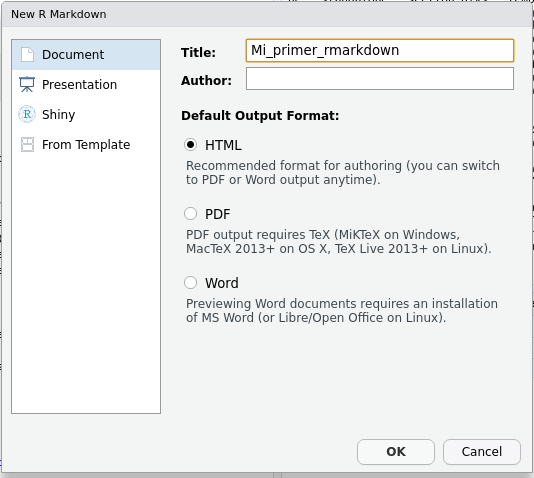
\includegraphics{img/nuevo-rmd.png}

Al aceptar, se abrirá un nuevo archivo con una plantilla de ejemplo (en
inglés).

\hypertarget{quarto}{%
\paragraph{Quarto}\label{quarto}}

Un archivo de Quarto (generalmente con la extensión \texttt{.qmd}), a
diferencia de un script \texttt{.R}, es un archivo de texto plano que
combina código de R que genera resultados (gráficos, tablas, etc\ldots)
y el texto que lo describe. Al poder intercalar cálculos y gráficos con
su análisis o explicación, se unifica el flujo de trabajo y deja de ser
necesario guardar figuras o tablas para luego insertarlas en un
documento de texto. Esto es muy importante si buscamos que nuestro
trabajo sea reproducible, pero además ahorra tiempo. Una ventaja por
sobre R Markdown es que Quarto es independiente del lenguaje de
programación. En este caso estamos usando R y RStudio pero podríamos
trabajar con python y notebooks de jupyter y aprovechar Quarto.

\hypertarget{creando-archivos-.qmd}{%
\subsubsection{Creando archivos .qmd}\label{creando-archivos-.qmd}}

En RStudio podés crear un nuevo archivo de Quarto con el menú
desplegable:

\begin{tcolorbox}[enhanced jigsaw, arc=.35mm, title=\textcolor{quarto-callout-note-color}{\faInfo}\hspace{0.5em}{Instrucciones}, coltitle=black, bottomrule=.15mm, breakable, colbacktitle=quarto-callout-note-color!10!white, bottomtitle=1mm, opacityback=0, toptitle=1mm, left=2mm, opacitybacktitle=0.6, rightrule=.15mm, toprule=.15mm, colback=white, colframe=quarto-callout-note-color-frame, leftrule=.75mm, titlerule=0mm]
File → New File → Quarto Document
\end{tcolorbox}

Y se abrirá un menú donde podés agregar el título de tu informe y tu
nombre. Por ahora vamos a usar el formato HTML como salida, pero hay
muchos otros formatos de salida posibles.

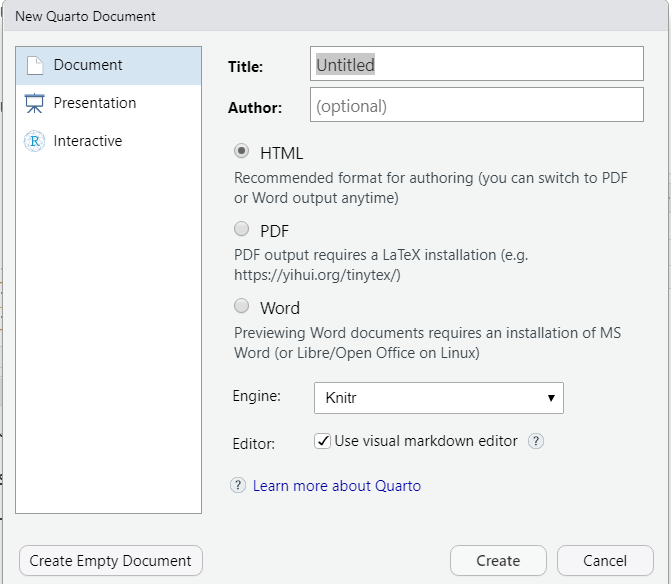
\includegraphics{img/nuevo-qmd.png}

Al aceptar, se abrirá un nuevo archivo con una plantilla de ejemplo (en
inglés).

\begin{tcolorbox}[enhanced jigsaw, arc=.35mm, title=\textcolor{quarto-callout-tip-color}{\faLightbulb}\hspace{0.5em}{Ejercicio}, coltitle=black, bottomrule=.15mm, breakable, colbacktitle=quarto-callout-tip-color!10!white, bottomtitle=1mm, opacityback=0, toptitle=1mm, left=2mm, opacitybacktitle=0.6, rightrule=.15mm, toprule=.15mm, colback=white, colframe=quarto-callout-tip-color-frame, leftrule=.75mm, titlerule=0mm]
\textbf{Primer desafío: Creá un nuevo archivo R Markdown}

Revisá la plantilla que trae el documento. ¿Podés identificar los
bloques de código?
\end{tcolorbox}

Para generar el archivo de salida, el paquete \textbf{knitr} (que viene
de \emph{tejer} en inglés) ejecutará el código en una sesión
independiente de R e interpretará el texto, su formato y cualquier otra
cosa que agreguemos (por ejemplo imágenes o links externos). Esto
significa que nuestro archivo debe tener \textbf{todo} lo necesario para
generar el análisis y si nos olvidamos de algo va a dar error.

Por esta razón es recomendable \emph{knitear} o \emph{renderizar} el
archivo seguido, para encontrarnos con los errores a tiempo y de paso
asegurarnos que el análisis es reproducible.

\begin{tcolorbox}[enhanced jigsaw, arc=.35mm, title=\textcolor{quarto-callout-tip-color}{\faLightbulb}\hspace{0.5em}{Ejercicio}, coltitle=black, bottomrule=.15mm, breakable, colbacktitle=quarto-callout-tip-color!10!white, bottomtitle=1mm, opacityback=0, toptitle=1mm, left=2mm, opacitybacktitle=0.6, rightrule=.15mm, toprule=.15mm, colback=white, colframe=quarto-callout-tip-color-frame, leftrule=.75mm, titlerule=0mm]
\textbf{Segundo desafío: renderizá tu documento de R Markdown}

Aprovechando la plantilla de RStudio, obtené el archivo de salida en
formato HTML haciendo click en el botón \textbf{Render} (el que tiene
una flecha celeste que apunta a la derecha!).
\end{tcolorbox}

\hypertarget{estructura-de-un-.rmd}{%
\subsection{Estructura de un .Rmd}\label{estructura-de-un-.rmd}}

Cualquier archivo de este tipo tiene 3 partes principales:

\begin{itemize}
\tightlist
\item
  El \textbf{encabezado o \emph{yaml}} que determina que pinta tendrá el
  archivo de salida, por ejemplo en formato html. También se puede
  incluir información sobre el autor, la fecha, si queremos o no una
  tabla de contenidos y muchas cosas más. Hay pequeñas diferencias entre
  R Markdown y Quarto.
\item
  El \textbf{texto o prosa} ya que puede estar a lo largo de todo el
  documento. Para darle formato a los títulos o por ejemplo resaltar
  parte del texto usando negrita se usa Markdown, un lenguaje que a
  diferencia de html es legible aún si no está compilado o en su versión
  final.
\item
  El \textbf{código en bloques o \emph{chuncks}}. Dentro de un chunk el
  código de R puede ejecutarse al igual que en un script normal y
  cualquier comentario o explicación debe tener al principio un
  \texttt{\#} para que R lo interprete correctamente.
\end{itemize}

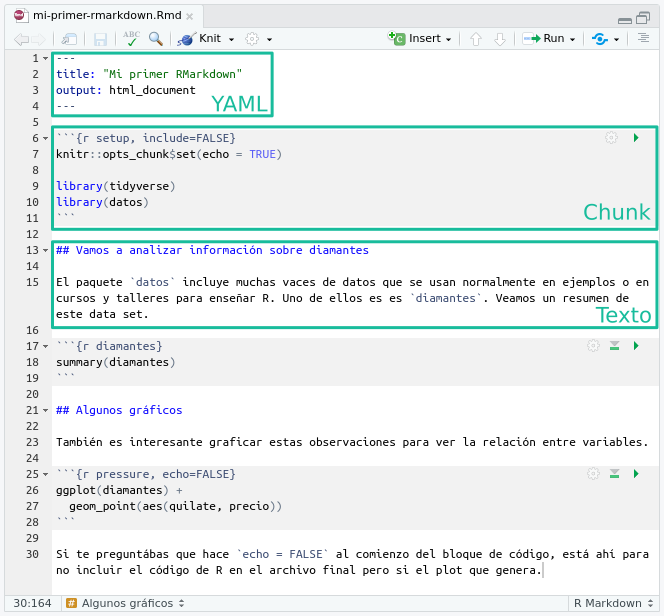
\includegraphics{img/rmd-ejemplo-secciones.png}

\hypertarget{encabezado}{%
\subsubsection{Encabezado}\label{encabezado}}

El encabezado es una serie de instrucciones organizadas entre tres
guiones (\texttt{-\/-\/-}) que determinan las propiedades globales del
documento, como el título, el formato de salida, información de autoría,
etc\ldots{} También ahí se pueden cambiar opciones asociadas al formato
de salida, como el estilo de la tabla de contenidos o índice.

Éstas propiedades se definen en un formato llamado
\href{https://es.wikipedia.org/wiki/YAML}{YAML}, el cual permite definir
listas jerarquizadas de una forma humanamente legible. Por ejemplo:

\begin{Shaded}
\begin{Highlighting}[]
\PreprocessorTok{{-}{-}{-}}
\FunctionTok{title}\KeywordTok{:}\AttributeTok{ }\StringTok{"Mi primer RMarkdown"}
\FunctionTok{output}\KeywordTok{:}\AttributeTok{ }
\AttributeTok{  }\FunctionTok{html\_document}\KeywordTok{:}
\AttributeTok{    }\FunctionTok{code\_download}\KeywordTok{:}\AttributeTok{ }\CharTok{true}
\AttributeTok{    }\FunctionTok{toc}\KeywordTok{:}\AttributeTok{ }\CharTok{true}
\AttributeTok{    }\FunctionTok{toc\_float}\KeywordTok{:}\AttributeTok{ }\CharTok{false}
\PreprocessorTok{{-}{-}{-}}
\end{Highlighting}
\end{Shaded}

define dos variables principales, ``title'' y ``output''. ``Output'' a
su vez contiene un elemento ``htm\_document'', el cual contiene tres
elementos: ``code\_download'', ``toc'' y ``toc\_float''.

\begin{tcolorbox}[enhanced jigsaw, arc=.35mm, title=\textcolor{quarto-callout-important-color}{\faExclamation}\hspace{0.5em}{Importante}, coltitle=black, bottomrule=.15mm, breakable, colbacktitle=quarto-callout-important-color!10!white, bottomtitle=1mm, opacityback=0, toptitle=1mm, left=2mm, opacitybacktitle=0.6, rightrule=.15mm, toprule=.15mm, colback=white, colframe=quarto-callout-important-color-frame, leftrule=.75mm, titlerule=0mm]
Es muy importante mantener el escalonado, o \emph{identación} de los
elementos, ya que ésta define la jerarquía de cada elemento. Muchos de
los errores a la hora de knitear ocurren porque el archivo tiene
problemas en la identación del encabezado.
\end{tcolorbox}

\hypertarget{bloques-de-cuxf3digo}{%
\subsubsection{Bloques de código}\label{bloques-de-cuxf3digo}}

El código de R que va a leer datos, analizarlos y generar figuras,
tablas o números se organiza en bloques (o \texttt{chunks}) delimitados
por tres acentos graves
(\texttt{\textasciigrave{}\textasciigrave{}\textasciigrave{}}) y se
diferencia del resto de archivo con un fondo gris. Todo lo que incluyas
entre estos delimitadores será interpretado por R como código e
intentará ejecutarlo al \emph{knitear} el archivo. Cualquier resultado
del código (gráficos, tablas, texto, etc\ldots) será insertado en el
documento final en el mismo orden que están en el archivo R Markdown.

\begin{tcolorbox}[enhanced jigsaw, arc=.35mm, title=\textcolor{quarto-callout-note-color}{\faInfo}\hspace{0.5em}{Instrucciones}, coltitle=black, bottomrule=.15mm, breakable, colbacktitle=quarto-callout-note-color!10!white, bottomtitle=1mm, opacityback=0, toptitle=1mm, left=2mm, opacitybacktitle=0.6, rightrule=.15mm, toprule=.15mm, colback=white, colframe=quarto-callout-note-color-frame, leftrule=.75mm, titlerule=0mm]

Para insertar un nuevo chunk podés:

\begin{itemize}
\tightlist
\item
  Usar el botón \textbf{Insert}
\item
  El atajo de teclado Ctrl+Alt+I
\item
  Escribir a mano!
\end{itemize}

\end{tcolorbox}

El código en cada bloque se ejecuta como si fuera ejecutado en la
terminal y todo resultado se muestra en el documento (ya vamos a ver
formas de controlar esto). Por ejemplo, este bloque de código

\begin{verbatim}
```{r sumar}
1 + 1
```
\end{verbatim}

va a insertar esto en el documento de salida:

\begin{verbatim}
[1] 2
\end{verbatim}

\begin{tcolorbox}[enhanced jigsaw, arc=.35mm, title=\textcolor{quarto-callout-important-color}{\faExclamation}\hspace{0.5em}{Importante}, coltitle=black, bottomrule=.15mm, breakable, colbacktitle=quarto-callout-important-color!10!white, bottomtitle=1mm, opacityback=0, toptitle=1mm, left=2mm, opacitybacktitle=0.6, rightrule=.15mm, toprule=.15mm, colback=white, colframe=quarto-callout-important-color-frame, leftrule=.75mm, titlerule=0mm]
Es muy importante no romper los límites de los bloques. Un problema
común es accidentalmente eliminar un acento grave al final de un bloque
de código y que luego el documento no knitee correctamente. Si al
knitear te sale un error como ``attempt to use zero-length variable
name'', revisá bien que todos tus bloques de código estén correctamente
definidos.
\end{tcolorbox}

Los bloques pueden tener nombre, lo cual es útil para identificar donde
ocurren los errores al momento de \emph{knitear} pero también para tener
una pista de lo que hace el código que incluye.

Si bien el código se corre cuando uno knitea, cuando estés escribiendo
un informe es muy cómodo ir corriendo bloques individuales
interactivamente como si fuera en la consola.

Para correr una línea de código, tendrás que pararte sobre esa línea y
apretar:

\begin{tcolorbox}[enhanced jigsaw, arc=.35mm, title=\textcolor{quarto-callout-note-color}{\faInfo}\hspace{0.5em}{Instrucciones}, coltitle=black, bottomrule=.15mm, breakable, colbacktitle=quarto-callout-note-color!10!white, bottomtitle=1mm, opacityback=0, toptitle=1mm, left=2mm, opacitybacktitle=0.6, rightrule=.15mm, toprule=.15mm, colback=white, colframe=quarto-callout-note-color-frame, leftrule=.75mm, titlerule=0mm]
Ctrl+Enter
\end{tcolorbox}

Pero también podés correr el código de todo el chunk con:

\begin{tcolorbox}[enhanced jigsaw, arc=.35mm, title=\textcolor{quarto-callout-note-color}{\faInfo}\hspace{0.5em}{Instrucciones}, coltitle=black, bottomrule=.15mm, breakable, colbacktitle=quarto-callout-note-color!10!white, bottomtitle=1mm, opacityback=0, toptitle=1mm, left=2mm, opacitybacktitle=0.6, rightrule=.15mm, toprule=.15mm, colback=white, colframe=quarto-callout-note-color-frame, leftrule=.75mm, titlerule=0mm]
Ctrl+Shift+Enter
\end{tcolorbox}

Los resultados van a aparecer inmediatamente debajo del bloque.

\begin{tcolorbox}[enhanced jigsaw, arc=.35mm, title=\textcolor{quarto-callout-tip-color}{\faLightbulb}\hspace{0.5em}{Ejercicio}, coltitle=black, bottomrule=.15mm, breakable, colbacktitle=quarto-callout-tip-color!10!white, bottomtitle=1mm, opacityback=0, toptitle=1mm, left=2mm, opacitybacktitle=0.6, rightrule=.15mm, toprule=.15mm, colback=white, colframe=quarto-callout-tip-color-frame, leftrule=.75mm, titlerule=0mm]

\textbf{Tercer desafío: Sumá un chunk a tu archivo}

Usando el archivo con el que venís trabajando insertá un nuevo chunk y:

\begin{enumerate}
\def\labelenumi{\arabic{enumi}.}
\tightlist
\item
  Cargá el paquete readr.
\item
  Creá una variable que se llame \texttt{variable\_prueba} y asignale un
  valor.
\item
  Mostrá ese valor.
\item
  Volvé a \emph{knitear} el archivo para ver el resultado
\end{enumerate}

\end{tcolorbox}

Finalmente, es posible que te encuentres mencionando resultados en el
texto, por ejemplo algo así como ``el promedio de la variable estudiada
es 3.45''. Y también es posible que ese valor cambie si utilizas una
base de datos distinta o si luego generas un informe pero para un mes
siguiente. Las chances de de que te olvides de actualizar ese ``3.45''
son super altas, por eso R Markdown también tiene la posibilidad de
incorporar código en línea con el texto.

Si tenés una una variable \texttt{promedio} que vale ``3.45'':

Para mencionarla en el texto entonces escribirías:

\begin{quote}
el promedio de la variable estudiada es `\texttt{r} \texttt{promedio}`.
\end{quote}

y el resultado en el documento kniteado sería

\begin{quote}
el promedio de la variable estudiada es 3.45.
\end{quote}

prueba: \texttt{3.45}

\hypertarget{el-texto-propio-del-documento.}{%
\subsubsection{El texto propio del
documento.}\label{el-texto-propio-del-documento.}}

Este es el texto dirigido a las personas que van a leer el reporte.
Incluirá una introducción, descripción de los datos y de los resultados;
es lo que escribirías en el archivo de Word.

A diferencia de Word, el formato del texto se define usando
\href{https://es.wikipedia.org/wiki/Markdown}{markdown}, que es un
lenguaje simple que permite indicar si un texto va en negrita, cursiva,
es un título, etc\ldots usando símbolos especiales dentro del texto.

\hypertarget{markdown}{%
\subsection{Markdown}\label{markdown}}

Markdown permite escribir en texto plano pero definiendo el formato
usando símbolos. Por ejemplo podés resaltar con \textbf{negrita} usando
dos asteriscos así: \texttt{**negrita**} o \emph{italizada} con un
asterisco de cada lado: \texttt{*itálicas*}.

También podés hacer una lista de elementos utilizando asteriscos:

\begin{verbatim}
* la negrita se consigue con dos asteriscos
* la italizada con un asterisco
* y para resaltar código se usa el acento grave `
\end{verbatim}

o guiones medios:

\begin{verbatim}
- la negrita se consigue con dos asteriscos
- la italizada con un asterisco
- y para resaltar código se usa el acento grave `
\end{verbatim}

Ambas listas se van a ver de esta manera:

\begin{itemize}
\tightlist
\item
  la negrita se consigue con dos asteriscos
\item
  la italizada con un asterisco
\item
  y para resaltar código se usa el acento grave `
\end{itemize}

Si en realidad querés una lista numerada, simplemente comenzá el renglón
un número y un punto. Podrías usar siempre el mismo número, markdown se
encarga del resto:

\begin{verbatim}
1. la negrita se consigue con dos asteriscos
1. la italizada con un asterisco
1. y para resaltar código se usa el acento grave `
\end{verbatim}

Ahora la lista numerada se ve así:

\begin{enumerate}
\def\labelenumi{\arabic{enumi}.}
\tightlist
\item
  la negrita se consigue con dos asteriscos
\item
  la italizada con un asterisco
\item
  y para resaltar código se usa el acento grave `
\end{enumerate}

Podés agregar títulos con distinta jerarquía agregando \texttt{\#} al
comienzo. Esto además define secciones dentro del documento:

\begin{verbatim}
# Título
## El primer subtítulo
### Otro subtítulo de menor jerarquía
#### Otro más, y podría seguir!
\end{verbatim}

Podés escribir estos símbolos a mano o usando el Editor Visual de
RStudio y cambiar de la versión código fuente a la versión visual según
prefieras (
\includegraphics{img/icono-editor-visual.png}) . El Editor
Visual permite dar formato al texto usando markdown sin saber usar
markdown.

\begin{tcolorbox}[enhanced jigsaw, arc=.35mm, title=\textcolor{quarto-callout-tip-color}{\faLightbulb}\hspace{0.5em}{Ejercicio}, coltitle=black, bottomrule=.15mm, breakable, colbacktitle=quarto-callout-tip-color!10!white, bottomtitle=1mm, opacityback=0, toptitle=1mm, left=2mm, opacitybacktitle=0.6, rightrule=.15mm, toprule=.15mm, colback=white, colframe=quarto-callout-tip-color-frame, leftrule=.75mm, titlerule=0mm]
\textbf{Cuarto desafío: Agregale texto a tu archivo}

Borrá el contenido del archivo \texttt{.Rmd} que creaste (pero no el
encabezado!) y probá escribir algo y darle formato. Luego volvé a
apretar el botón \textbf{knit} para ver el resultado.
\end{tcolorbox}

Markdown permite muchas otras cosas, por ejemplo:

\begin{itemize}
\item
  Podés agregar un link a una página externa:
  \texttt{{[}texto\ que\ se\ muestra\ con\ el\ link{]}(http://google.com)}.
  Resultado: \href{http://google.com}{texto que se muestra con el link}
\item
  Podés incluir una imagen:
  \texttt{!{[}descripción\ de\ la\ figura{]}(https://placekitten.com/200/100)}
\end{itemize}

Resultado:

\begin{figure}

{\centering \includegraphics{img/kitty100.jpeg}

}

\caption{descripción de la figura}

\end{figure}

Y también podés agregar ecuaciones (usando
\href{https://es.wikipedia.org/wiki/LaTeX}{LaTeX}) en la misma línea
(esto:\texttt{\$E\ =\ mc\^{}2\$} se ve así: \(E = mc^2\)) o en una línea
propia. Esto:

\begin{verbatim}
$$
y = \mu + \sum_{i=1}^p \beta_i x_i + \epsilon
$$
\end{verbatim}

se ve así:

\[
y = \mu + \sum_{i=1}^p \beta_i x_i + \epsilon
\]

\begin{tcolorbox}[enhanced jigsaw, arc=.35mm, title=\textcolor{quarto-callout-note-color}{\faInfo}\hspace{0.5em}{Información}, coltitle=black, bottomrule=.15mm, breakable, colbacktitle=quarto-callout-note-color!10!white, bottomtitle=1mm, opacityback=0, toptitle=1mm, left=2mm, opacitybacktitle=0.6, rightrule=.15mm, toprule=.15mm, colback=white, colframe=quarto-callout-note-color-frame, leftrule=.75mm, titlerule=0mm]
Podés revisar la guía rápida de Markdown desde RStudio (en inglés):

Help → Markdown Quick Reference
\end{tcolorbox}



\end{document}
